%% ===================================================================
%%  GenoFold -- IEEE BIBM 2026 Undergraduate & High School Symposium
%%  Camera-ready revision (5-page limit, high-school first author).
%%  Addresses the two reviewer reports; see README.md for the mapping.
%%
%%  Build:  latexmk -pdf ughs.tex
%% ===================================================================

\documentclass[conference]{IEEEtran}
\IEEEoverridecommandlockouts

\usepackage{cite}
\usepackage{amsmath,amssymb,amsfonts}
\usepackage{graphicx}
\usepackage{textcomp}
\usepackage{xcolor}
\usepackage{booktabs}
\usepackage{balance}
\usepackage[hidelinks,breaklinks=true]{hyperref}

\begin{document}

\title{GenoFold: A Multi-Modal Graph--Transformer Reconstructor of\\ 3D Genome
Architecture with Per-Bin Uncertainty}

\author{%
\IEEEauthorblockN{Ram S. Seelamankalugari}
\IEEEauthorblockA{\textit{High School Student}\\
\textit{SYALIS Labs}\\
Frisco, Texas, United States \\
ramresearch.sa@gmail.com}
\and
\IEEEauthorblockN{Quang Bui}
\IEEEauthorblockA{\textit{Synthica Research Group}\\
\textit{American International School Vienna}\\
Vienna, Austria \\
quangbui@mit.edu}
}

\maketitle

% -------------------------------------------------------------------
\begin{abstract}
Most methods that rebuild chromosome structure from Hi-C use the contact
matrix alone and solve each matrix from scratch. GenoFold is a trained
reconstructor whose genomic bins carry sequencing coverage, 4-mer
composition, GC content and mappability alongside Hi-C contacts; a
four-layer GATv2 encoder and a six-layer Transformer feed a coordinate
decoder trained with a self-supervised distance-matching loss. On dense
GM12878 Hi-C it does not beat existing methods: its distance Spearman
correlation (dSCC) on chromosome~22 is $0.893 \pm 0.001$, against 0.900
for 3DMax and 0.889 for HiC-GNN, and the gaps are of the order of
run-to-run variation. Scored against distances measured by chromatin
tracing in IMR90 and K562, GenoFold reaches Spearman 0.986 and 0.981. When
contacts are downsampled to 5\%, it still reaches 0.978 and 0.969 while
3DMax falls to 0.819 and 0.831. A modality ablation shows that only a
small part of this gap comes from the extra node features; most of it
appears to come from the structural prior the trained decoder has
learned. A per-bin uncertainty estimate ranks reconstruction error only
weakly (Spearman 0.28), and we report it as such.
\end{abstract}

\begin{IEEEkeywords}
3D genome reconstruction, Hi-C, graph attention networks, multi-modal
learning, uncertainty estimation
\end{IEEEkeywords}

% ===================================================================
\section{Introduction}

Chromatin folding decides which enhancers can contact their promoters and
where topologically associating domains (TADs) begin and
end~\cite{lieberman2009,dixon2012}. Hi-C measures how often pairs of loci
are ligated together~\cite{rao2014}, and a family of methods converts
those frequencies into coordinates. 3DMax optimizes coordinates by
maximum likelihood with contact frequency standing in for
distance~\cite{oluwadare2018}; ShRec3D embeds shortest-path distances by
multidimensional scaling~\cite{lesne2014}; FLAMINGO completes sparse
high-resolution matrices with a low-rank model~\cite{flamingo2022};
HiC-GNN learns node embeddings with a graph neural
network~\cite{hicgnn2022}. All four read Hi-C and nothing else, and all
but HiC-GNN fit each matrix independently, so a shallow library gives
them little to work with.

GenoFold~\cite{genofold2025} tests whether two additions help: node
features that do not depend on sequencing depth (coverage, sequence
composition, GC content and mappability), and a trained network that can
carry structure learned on one matrix into another. Our claims are
narrower than in the submitted version. We contribute (i) a trained
GATv2--Transformer reconstructor that matches established methods on
dense Hi-C; (ii) validation against measured chromatin-tracing distances,
which are independent of the training signal; (iii) a sparse-contact
experiment in which GenoFold degrades far less than per-matrix
optimizers, together with an ablation that attributes most of that
robustness to the learned prior rather than to the added modalities; and
(iv) a per-bin uncertainty estimate and feature-group attributions,
whose limits we state.

% ===================================================================
\section{Method}

\textit{Preprocessing.} Bins whose row-wise zero fraction exceeds 0.97
are removed; the threshold is looser than the usual 0.8 so that sparse
pericentromeric bins are kept. Matrices are balanced by ICE
(tolerance $10^{-5}$)~\cite{imakaev2012}. Coverage is RPKM-normalized,
corrected for GC bias and mappability, and z-scored; GC content comes
from hg19 and mappability from the ENCODE/CRG 50-mer track.

\textit{Graph.} Each chromosome becomes a graph with $M$ nodes. A node
carries 140 features: coverage (1), reverse-complement-collapsed 4-mer
frequencies (136), GC and mappability (2), and normalized position (1).
Edges carry the log contact weight and log genomic distance, stored as a
PyTorch Geometric object~\cite{pyg2019}.

\begin{table}[t]
\caption{Node features ($F=140$). Only the coverage track depends on
sequencing depth; contacts enter through the edges.}
\label{tab:features}
\centering
\begin{tabular}{@{}lcl@{}}
\toprule
Group & Dim & Source \\
\midrule
Coverage & 1 & RPKM read depth, GC/mappability-corrected \\
Sequence & 136 & RC-collapsed 4-mer frequencies (hg19) \\
Metadata & 2 & GC content; CRG 50-mer mappability \\
Position & 1 & Normalized bin index \\
\bottomrule
\end{tabular}
\end{table}

\textit{Encoder and decoder.} Four GATv2 layers~\cite{brody2022} (8 heads
with residual connections in the first three, 4 averaged heads in the
last, $d=64$) supply local context. Six pre-norm Transformer
layers~\cite{vaswani2017} (8 heads, FFN width 512, GELU, dropout 0.1)
add interactions between all pairs of bins. A five-layer MLP
($64\!\to\!128\!\to\!256\!\to\!128\!\to\!3$) decodes coordinates. The
code also contains a species embedding; every experiment here uses one
species, so the embedding holds a single constant value and has no
effect. We do not count it as part of the method. The model has 2.71~M
parameters.

\textit{Objective.} Contacts map to wish distances
$D_{ij}=C_{ij}^{-0.25}$, and the network minimizes
\begin{equation}
\mathcal{L}=\frac{1}{|P|}\sum_{(i,j)\in P}\big(\hat z_{ij}-z^{*}_{ij}\big)^2
+\lambda\,\mathcal{L}_{\mathrm{NLL}},
\end{equation}
where $\hat z_{ij}$ and $z^{*}_{ij}$ are z-scored log reconstructed and
wish distances over observed pairs $P$, and $\mathcal{L}_{\mathrm{NLL}}$
is a Gaussian negative log-likelihood that trains the variance head. We
use Adam (learning rate $10^{-3}$, cosine schedule, weight decay
$10^{-5}$) for 300 epochs. Held-out dSCC on a 20\% pair holdout levels
off by epoch 150 and moves by less than 0.002 over the last 50 epochs.
No early stopping is used; all results come from the epoch-300
checkpoint. Held-out dSCC (0.890) and training dSCC (0.890) differ by
less than 0.001, so the model is not fitting individual pairs. A
per-matrix optimizer such as 3DMax has no counterpart to this test,
since it fits every observed pair by construction.

\textit{Uncertainty.} The variance head predicts per-axis log-variances
$v_{ik}$; $T$ Monte Carlo dropout passes~\cite{gal2016} add an epistemic
term. The per-bin radius is
$r_i=(\sum_k\sigma_{ik}^2)^{1/2}$ with $\sigma_{ik}=\exp(v_{ik}/2)$.

\textit{Attribution.} Integrated Gradients~\cite{sundararajan2017} (32
steps from a zero baseline) are summed within each of the four feature
groups. TADs are called on reconstructions by insulation
score~\cite{crane2015}.

% ===================================================================
\section{Experimental Setup}

We use the Rao et al.\ \textit{in situ} Hi-C maps for GM12878, IMR90 and
K562 (GSE63525, KR-normalized)~\cite{rao2014}. The main benchmark is
GM12878 chromosome~22 at 50~kb (701 bins after filtering), scored by
dSCC, the Spearman correlation between reconstructed and wish distances
over observed pairs, and by TAD-boundary $F_1$. 3DMax, HiC-GNN and
ShRec3D are re-implemented on the identical submatrix; FLAMINGO runs from
its published R package. Means and standard deviations are over three
seeds.

For a check that does not reuse the training signal we take the
chromatin-tracing data of Bintu et al.~\cite{bintu2018}: median pairwise
distances between 65 consecutive 30~kb segments of chromosome~21 (hg19
chr21:29.37--31.32~Mb), imaged in thousands of IMR90 and K562 cells. Each
method reconstructs the region from the matched 10~kb Hi-C; coordinates
are coarse-grained onto the imaging grid and correlated with the imaged
medians. The tracing coordinates are annotated on hg38; we register them
to the hg19 Hi-C by the liftOver offset ($+1.37$~Mb) that maximizes
agreement between raw Hi-C and imaging, and apply the same registration
to every method. For the sparse experiments, each contact matrix is
thinned by keeping a random fraction of its nonzero bin pairs (values
unchanged, symmetry preserved); each method then reconstructs from the
thinned matrix alone. This removes pairs rather than reads, so it
mimics loss of coverage more crudely than read-level subsampling.

% ===================================================================
\section{Results}

\subsection{Dense Hi-C}
Table~\ref{tab:benchmark} gives the GM12878 benchmark. 3DMax has the
highest dSCC (0.900); GenoFold (0.893) and HiC-GNN (0.889) follow, and
the differences are of the same size as the 0.01--0.02 spread we see
between runs. We do not read them as a ranking. GenoFold is also the
slowest method (245~s on CPU), most of it spent in the $O(M^2)$
Transformer attention and the dropout passes.

FLAMINGO is built for 1--5~kb data, and at 50~kb its dSCC is 0.27, which
says more about the setting than the method; we therefore leave it out of
Table~\ref{tab:benchmark}. At its native 5~kb, on chr22:20--30~Mb (1{,}964
bins), FLAMINGO reaches 0.655 (Table~\ref{tab:5kb}), against 0.820 for 3DMax, 0.814 for GenoFold
and 0.783 for ShRec3D. These dSCC numbers favour the all-pair optimizers,
since dSCC is close to their objective and not to FLAMINGO's.

\begin{table}[t]
\caption{Native-resolution comparison at 5~kb on chr22:20--30~Mb (1{,}964
bins). Short-range: pairs $\le$1~Mb apart. $^{\ast}$FLAMINGO from its R
package, 3 seeds; others single runs.}
\label{tab:5kb}
\centering
\begin{tabular}{@{}lcc@{}}
\toprule
Method & Global dSCC & Short-range dSCC \\
\midrule
3DMax & \textbf{0.820} & \textbf{0.895} \\
GenoFold & 0.814 & 0.892 \\
ShRec3D & 0.783 & 0.677 \\
FLAMINGO$^{\ast}$ & $0.655\pm0.017$ & 0.667 \\
\bottomrule
\end{tabular}
\end{table}

\begin{table}[t]
\caption{GM12878 chr22, 50~kb, 701 bins (mean $\pm$ s.d., 3 seeds;
ShRec3D is deterministic). Time is CPU wall-clock per run.}
\label{tab:benchmark}
\centering
\setlength{\tabcolsep}{4pt}
\begin{tabular}{@{}lccc@{}}
\toprule
Method & dSCC & TAD $F_1$ & Time (s) \\
\midrule
ShRec3D  & 0.887 & 0.45 & 1.4 \\
3DMax    & $\mathbf{0.900}\pm0.000$ & $0.59\pm0.01$ & 29.1 \\
HiC-GNN  & $0.889\pm0.002$ & $\mathbf{0.60}\pm0.01$ & 100.6 \\
GenoFold & $0.893\pm0.001$ & $0.57\pm0.01$ & 244.9 \\
\bottomrule
\end{tabular}
\end{table}

\textit{Other chromosomes.} The full baseline suite has so far been run
only on chromosome~22. For GenoFold alone, whole-chromosome runs give
dSCC 0.891 on chr22 (701 bins), 0.880 on chr20 (1{,}196) and 0.865 on
chr16 (1{,}582); runtime rises from 223~s to 1{,}218~s and peak memory
from 1.7 to 3.7~GB (Table~\ref{tab:chrom}). Accuracy therefore declines slowly as chromosomes
grow, but without matching baseline runs these numbers say nothing about
relative standing. A per-chromosome comparison across all methods is the
first item of our follow-up work.

\begin{table}[t]
\caption{GenoFold on whole chromosomes of GM12878 at 50~kb (CPU).}
\label{tab:chrom}
\centering
\begin{tabular}{@{}lcccc@{}}
\toprule
Chrom. & Bins & dSCC & Time (s) & Peak RSS (GB) \\
\midrule
chr22 & 701 & 0.891 & 223 & 1.7 \\
chr20 & 1{,}196 & 0.880 & 632 & 2.8 \\
chr16 & 1{,}582 & 0.865 & 1{,}218 & 3.7 \\
\bottomrule
\end{tabular}
\end{table}

Fig.~\ref{fig:structure} shows the chr22 reconstruction next to the
observed contact map. The pseudo-contacts implied by the coordinates
reproduce the block structure of the observed map, though the
reconstruction smooths the sharpest domain corners.

\begin{figure}[t]
\centering
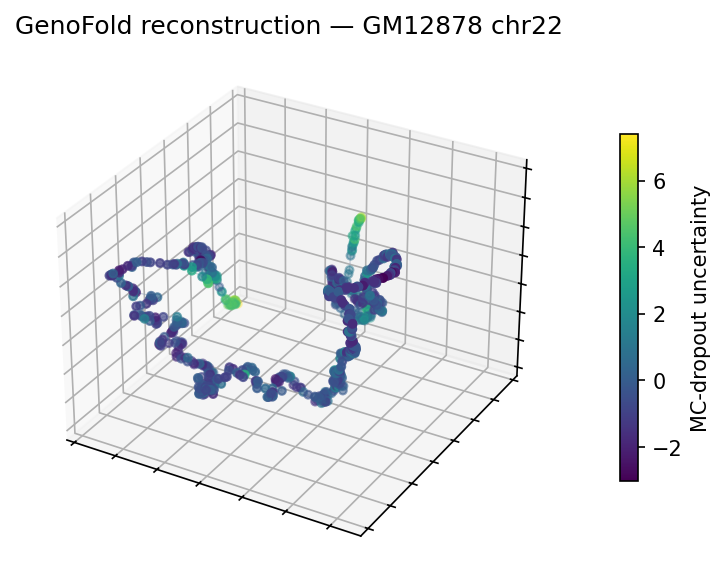
\includegraphics[width=0.49\columnwidth]{figures/fig_structure.png}\hfill
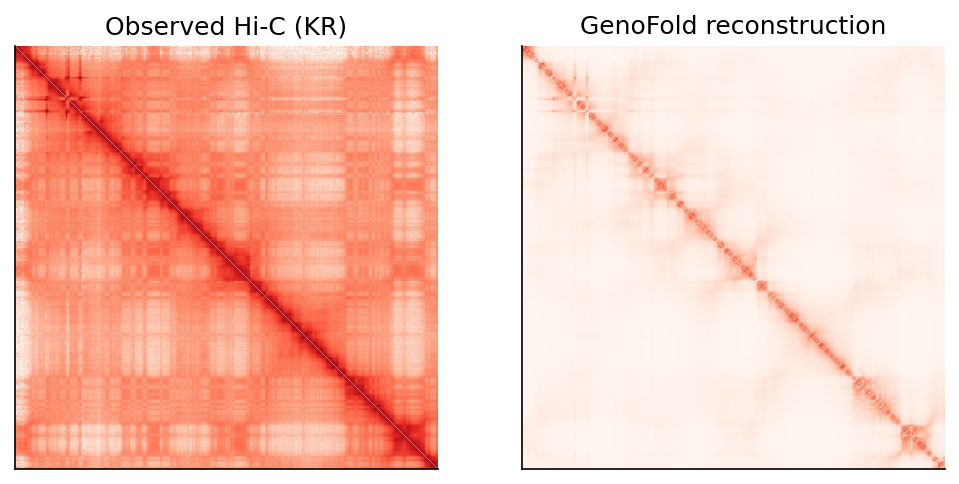
\includegraphics[width=0.49\columnwidth]{figures/fig_contact.png}
\caption{GM12878 chr22. Left: reconstruction coloured by per-bin
uncertainty. Right: observed KR-normalized contacts against the
pseudo-contacts implied by the reconstruction ($\log(1+x)$).}
\label{fig:structure}
\end{figure}

\subsection{Agreement with Measured Distances}
Table~\ref{tab:fish} compares reconstructed and imaged distances. At full
depth GenoFold (0.986, 0.981) and 3DMax (0.987, 0.979) are level, and both
exceed the raw Hi-C contacts read directly as distances (0.973, 0.963).
Because the imaging data were never used for training, this agreement is
evidence that the dSCC scores reflect physical structure and not only
consistency with the loss.

\begin{table}[t]
\caption{Spearman correlation with median chromatin-tracing distances
(chr21, 65 segments)~\cite{bintu2018} at full Hi-C depth and with 5\% of
contacts kept. GenoFold: mean of 3 seeds (s.d.\ $\le$0.004). Raw Hi-C
scores the (thinned) contacts as distances, with no reconstruction.}
\label{tab:fish}
\centering
\setlength{\tabcolsep}{4pt}
\begin{tabular}{@{}lcccc@{}}
\toprule
 & \multicolumn{2}{c}{IMR90} & \multicolumn{2}{c}{K562} \\
\cmidrule(lr){2-3}\cmidrule(l){4-5}
Method & 100\% & 5\% & 100\% & 5\% \\
\midrule
GenoFold   & 0.986 & \textbf{0.978} & \textbf{0.981} & \textbf{0.969} \\
3DMax      & \textbf{0.987} & 0.819 & 0.979 & 0.831 \\
ShRec3D    & 0.970 & 0.689 & 0.960 & 0.581 \\
Raw Hi-C   & 0.973 & 0.904 & 0.963 & 0.885 \\
\bottomrule
\end{tabular}
\end{table}

\subsection{Sparse Hi-C, and What Drives It}
We downsampled each cell line's contacts to 25\%, 10\% and 5\%,
reconstructed from the thinned matrix, and scored against the full-depth
imaging data (Fig.~\ref{fig:sparse}, Table~\ref{tab:fish}). GenoFold
changes by less than 0.02 across this range. 3DMax holds up to 10\%
(0.955, 0.948) and then drops to 0.819 and 0.831 at 5\%; ShRec3D drops
further. Below 10\% GenoFold's reconstructions agree with the imaging
data better than the thinned contacts themselves do.

Both reviewers asked whether this gap comes from the added modalities or
simply from having a trained model. Our own ablation points to the
second. On GM12878 chr22, a GenoFold variant with Hi-C-only nodes trails
the full model by only 0.002 dSCC at 50\% depth and 0.005 at 5\% (0.884
against 0.879), and at full depth every configuration lies within 0.01
(Hi-C only 0.889; without 4-mers 0.886; without GC and mappability
0.894). Table~\ref{tab:ablation} lists these runs. A margin that small cannot account for a 0.14--0.16 lead over
3DMax. The more likely explanation is that the decoder has learned what
chromatin at 10--50~kb tends to look like, which a per-matrix optimizer
cannot do. Two experiments would settle the question, and we have not
yet run either: the imaging comparison with a Hi-C-only GenoFold, and
the same comparison with HiC-GNN, the one trainable baseline, which is
missing from the sparse experiment. Until they are done we state the
sparse result as an advantage of a trained reconstructor, not of
multi-modality.

\begin{table}[t]
\caption{Modality ablation, GM12878 chr22 (held-out dSCC). Left: full
depth; ``sparse'' restricts to pairs touching the lowest-coverage third
of bins. Right: Hi-C-only versus full model as contacts are removed.}
\label{tab:ablation}
\centering
\setlength{\tabcolsep}{3pt}
\begin{tabular}{@{}lcc@{}}
\toprule
Configuration & All pairs & Sparse \\
\midrule
Full model & 0.890 & 0.871 \\
$-$ 4-mers & 0.886 & 0.867 \\
$-$ GC, mappability & 0.894 & 0.877 \\
Hi-C only & 0.889 & 0.871 \\
\bottomrule
\end{tabular}\hfill
\begin{tabular}{@{}lcc@{}}
\toprule
Depth & Full & Hi-C only \\
\midrule
50\% & 0.890 & 0.888 \\
20\% & 0.889 & 0.887 \\
10\% & 0.892 & 0.888 \\
5\% & 0.884 & 0.879 \\
\bottomrule
\end{tabular}
\end{table}

\begin{figure*}[t]
\centering
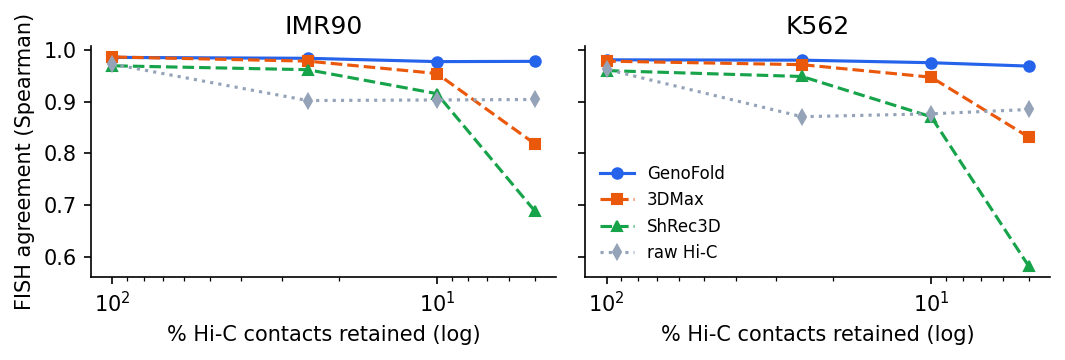
\includegraphics[width=0.8\textwidth]{figures/fig_fish_sparse.png}
\caption{Agreement with imaged chr21 distances as Hi-C contacts are
downsampled (log axis, right to left) in IMR90 and K562. GenoFold stays within 0.02 of its full-depth score;
3DMax and ShRec3D fall sharply below 10\% of contacts. Raw Hi-C scores
the thinned contacts as distances.}
\label{fig:sparse}
\end{figure*}

\subsection{Transfer Across Cell Lines}
Because GenoFold learns a mapping rather than a set of free coordinates,
a model trained on one matrix can be applied to another. Retrained on
IMR90 and K562 chr22, it reaches dSCC 0.795 and 0.754
(Table~\ref{tab:crosscell}). These scores are lower than on GM12878
mainly because the IMR90 and K562 libraries have roughly a fifth of
GM12878's read depth at this locus. A GM12878-trained model applied
without retraining gives 0.630 and 0.653: well above chance, but clearly
below retraining. Transfer is therefore a convenience for a quick first
structure, and retraining remains the better choice when a target
matrix is available.

\begin{table}[t]
\caption{Cross-cell-line results on chr22. Transfer applies the
GM12878-trained model unchanged; retrained fits the target line.}
\label{tab:crosscell}
\centering
\begin{tabular}{@{}lcc@{}}
\toprule
Cell line & Transfer dSCC & Retrained dSCC \\
\midrule
GM12878 (train) & \multicolumn{2}{c}{0.892 (in-domain)} \\
IMR90 & 0.630 & 0.795 \\
K562 & 0.653 & 0.754 \\
\bottomrule
\end{tabular}
\end{table}

\subsection{Uncertainty}
The combined per-bin radius correlates with per-bin reconstruction error
at Spearman 0.28 on chr22. Fig.~\ref{fig:calib} shows how that
correlation arises. Sorting bins into deciles of predicted uncertainty,
the mean error stays between 0.087 and 0.099 over the lowest nine
deciles and rises to 0.126 in the highest. The estimate thus flags the
worst tenth of bins and does little ranking among the rest. We have not
compared it with a simple proxy such as per-bin contact count, nor tested
whether the radii give the coverage their nominal intervals imply. Until
those tests exist the radius should be read as a coarse warning signal;
we no longer describe it as calibrated.

\begin{figure}[t]
\centering
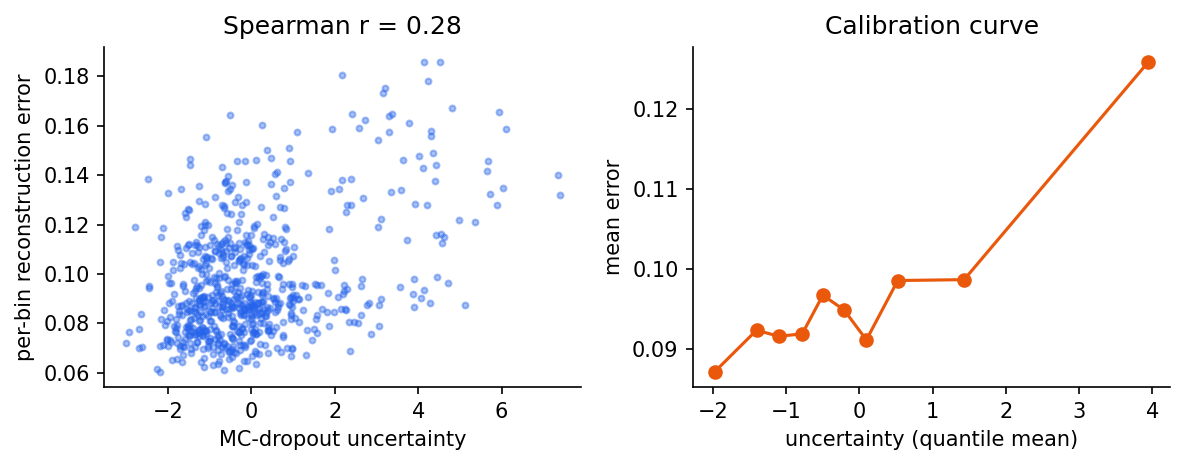
\includegraphics[width=\columnwidth]{figures/fig_calibration.png}
\caption{GM12878 chr22. Left: per-bin uncertainty against error.
Right: mean error by uncertainty decile.}
\label{fig:calib}
\end{figure}

\subsection{Attribution}
Integrated Gradients on the trained chr22 model, summed by feature group
and normalized (Fig.~\ref{fig:importance}), give 0.43 to GC and mappability, 0.30 to coverage, 0.18
to position and 0.10 to the 136 4-mer features. Two cautions apply.
Attribution measures sensitivity, and the ablation shows that removing
GC and mappability does not lower dSCC (0.894 against 0.890). The two
results are compatible: the model reads these features, but at full depth
the contact graph carries the same information. The attributions describe
what the network uses; they are not evidence that any modality is
needed.

\begin{figure}[t]
\centering
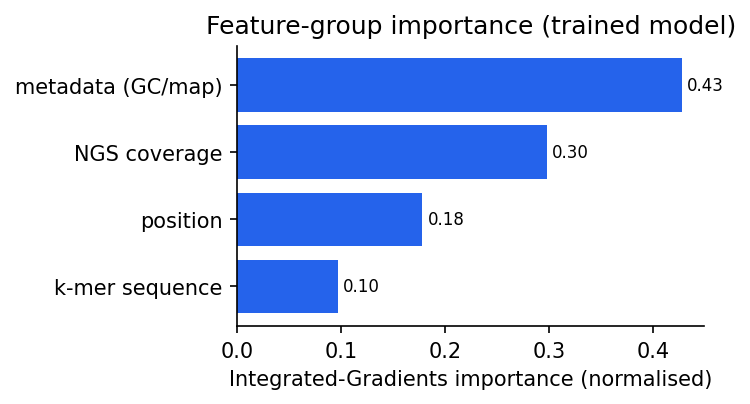
\includegraphics[width=0.9\columnwidth]{figures/fig_importance.png}
\caption{Integrated-Gradients importance by feature group, trained
GM12878 chr22 model.}
\label{fig:importance}
\end{figure}

% ===================================================================
\section{Discussion and Limitations}

On dense Hi-C, GenoFold is one of several methods that land within noise
of one another, and it is the slowest of them. Its case rests on shallow
data. There it keeps close to measured structure while per-matrix
optimizers lose it, but the evidence available now credits the learned
prior more than the added modalities, and a fair test against a trained
Hi-C-only model is still outstanding. The uncertainty estimate separates
only the least reliable bins, and the attribution results show
sensitivity rather than necessity.

Several limits remain. The objective trains on Hi-C-derived distances,
and the independent imaging check covers one 2~Mb region of one
chromosome. The comparison of all methods uses GM12878 chr22 only. All
cell lines are human, so nothing here tests the species embedding, which
is inactive. Bins kept by the 0.97 filter include low-mappability
regions where any reconstruction is weakly constrained.

\section{Conclusion}

GenoFold reconstructs chromatin structure from Hi-C and depth-independent
node features with accuracy level with 3DMax and HiC-GNN on dense data
and close to measured distances (Spearman 0.986 and 0.981). With 5\% of
contacts it stays at 0.978 and 0.969 where 3DMax falls to about 0.82, an
advantage we currently attribute to training rather than to
multi-modality. The next experiments are a Hi-C-only GenoFold and HiC-GNN
on the sparse imaging task, a per-chromosome benchmark, and coverage
tests for the uncertainty estimate. Code and checkpoints will be released
on acceptance.

\balance
\bibliographystyle{IEEEtran}
\bibliography{references}

\end{document}
